\chapter{Sysvinit 项目工具简介}

\section{项目背景介绍}

安装的程序 halt, init, killall5, last, lastb (链接到 last), mesg, pidof
(链接到 killall5), poweroff (链接到 halt), reboot (链接到 halt),
runlevel, shutdown, sulogin, telinit (链接到 init), utmpdump, wall
简要描述

\section{项目架构设计}

\chapter{Sysvinit 项目概要分析}

\section{工具安装使用流程}

Sysvinit软件包包含控制启动,运行和关闭所有其他程序的工具。

所有工具编译之后都生成在 src 源码目录树下,同时,这些命名的帮助文件在 man
目录下。

{\begin{shaded}\begin{verbatim}
$ ls -l
total 108
-rw-r--r-- 1 akaedu akaedu  2847 Jun 23 11:13 bootlogd.8
-rw-r--r-- 1 akaedu akaedu  1971 Jun 23 11:13 bootlogd.8.todo
-rw-r--r-- 1 akaedu akaedu  1444 Jun 23 11:13 fstab-decode.8
-rw-r--r-- 1 akaedu akaedu  3957 Jun 23 11:13 halt.8
-rw-r--r-- 1 akaedu akaedu 12124 Jun 23 11:13 init.8
-rw-r--r-- 1 akaedu akaedu  2428 Jun 23 11:13 initscript.5
-rw-r--r-- 1 akaedu akaedu  8290 Jun 23 11:13 inittab.5
-rw-r--r-- 1 akaedu akaedu  1866 Jun 23 11:13 killall5.8
-rw-r--r-- 1 akaedu akaedu  4242 Jun 23 11:13 last.1
-rw-r--r-- 1 akaedu akaedu    16 Jun 23 11:13 lastb.1
-rw-r--r-- 1 akaedu akaedu  1867 Jun 23 11:13 mesg.1
-rw-r--r-- 1 akaedu akaedu  1886 Jun 23 11:13 mountpoint.1
-rw-r--r-- 1 akaedu akaedu  3230 Jun 23 11:13 pidof.8
-rw-r--r-- 1 akaedu akaedu    16 Jun 23 11:13 poweroff.8
-rw-r--r-- 1 akaedu akaedu    16 Jun 23 11:13 reboot.8
-rw-r--r-- 1 akaedu akaedu  1872 Jun 23 11:13 runlevel.8
-rw-r--r-- 1 akaedu akaedu  8017 Jun 23 11:13 shutdown.8
-rw-r--r-- 1 akaedu akaedu  3309 Jun 23 11:13 sulogin.8
-rw-r--r-- 1 akaedu akaedu    16 Jun 23 11:13 telinit.8
-rw-r--r-- 1 akaedu akaedu  1949 Jun 23 11:13 utmpdump.1
-rw-r--r-- 1 akaedu akaedu  1960 Jun 23 11:13 wall.1
\end{verbatim}\end{shaded}}
通过使用 man 命令,加上 -l 参数,例如 man -l init.8
我们可以了解到这些命令的用法。

\begin{itemize}
\item
  注意
\end{itemize}
我们这里没有直接使用例如 man init 这样的命令,而是改用 man -l
init.8,这是因为前者是查看当前系统的帮助,而当前系统是 ubuntu 12.04
已经改用 upstart 作为 init 进程。后者才是针对 sysvinit
工具中的可执行文件配套的帮助信息。

下面我们针对这些命令的帮助信息,来给出每个命令的具体用法,在测试案例报告中,我们会详细说明每个命令如何使用。

\subsection{init 命令}

\subsubsection{init 命令说明}

init 进程是所有进程的父进程。它的主要任务就是从 /etc/inittab
文件中读取命令行,从而创建出一系列后继进程。 init 进程本身是被 Kernel
所启动,Kernel 将控制权交给它之后,用它来负责启动所有其他的进程。 inittab
文件中通常有关于登录接口的定义,就是在每个终端产生getty,使用户可以进行登录.

\subsubsection{命令格式}

{\begin{shaded}\begin{verbatim}
   /sbin/init [ -a ] [ -s ] [ -b ] [ -z xxx ] [ 0123456Ss ]
\end{verbatim}\end{shaded}}
\subsubsection{运行级别}

运行级别是Linux操作系统的一个软件配置,用它来决定启动哪些程序集来运行。
系统启动时,可以根据 /etc/inittab 文件的配置,进入不同的运行级别。
每个运行级别可以设置启动不同的程序。

启动的每个程序都是init的进程的子进程,运行级别有8个,分别是 0-6,S或s。
运行级别0,1和6是系统保留的。

\begin{itemize}
\item
  运行级别0用来关闭系统,
\item
  运行级别1先关闭所有用户进程和服务,然后进入单用户模式。
\item
  运行级别6用来重启系统。
\item
  运行级别S和s,会直接进入到单用户模式。
  \begin{itemize}
  \item
    这种模式下不再需要 /etc/inittab 文件。
  \item
    /sbin/sulogin 会在 /dev/console 上 被启动。
  \item
    运行级别S和s的功能是相同的。
  \end{itemize}
\end{itemize}
\subsubsection{启动过程}

在kernel启动的最后阶段,会调用init。init会查找/etc/inittab文件内容,进入指定的运行级别。
其中 initdefault
代表着系统默认要进入的运行级别,如果用户指定了,就会进入到 initdefault
代表的那个运行级别。 如果用户没有指定,则系统启动时,会通过 console
来要求用户输入一个运行级别。

当启动一个新进程时,init会先检查/etc/initscript文件是否存在。如果存在,则使用这个脚本来启动那个进程。

\subsubsection{选项}

\begin{itemize}
\item
  -s, S, single\\ 进入单用户模式.
\item
  1-5\\ 启动进入的运行级别.
\item
  -b, emergency\\ 直接进入单用户shell,不运行任何其他的启动脚本。
\item
  -a, auto\\ 如果指定该参数,init 会将 AUTOBOOT 环境变量设置为 yes。
\item
  -z xxx\\
  -z后面的参数将被忽略。可以使用这种方法将命令行加长一点,这样可以增加在堆栈中占用的空间。
\end{itemize}
\subsection{shutdown 命令}

\subsubsection{shutdown 命令说明}

shutdown
以一种安全的方式终止系统,所有正在登录的用户都会收到系统将要终止的通知,并且不准新的登录。

\subsubsection{命令格式}

\subsubsection{运行级别}

\subsubsection{启动过程}

\subsection{halt 命令}

\subsubsection{halt 命令说明}

halt 停止系统。通常以 -h 参数调用
shutdown,但如果已经在运行级0的话,它就告诉内核终止系统。在这之前,它会检查文件
/var/log/wtmp,看系统是否正在关闭。

正常情况下等效于 shutdown 加上 -h 参数(当前系统运行级别是 0
时除外)。它将告诉内核去中止系统,并在系统正在关闭的过程中将日志记录到
/var/log/wtmp 文件里。

\subsubsection{停止系统}

\subsubsection{主要选项:}

\begin{itemize}
\item
  -n\\ reboot或者halt之前,不同步(sync)数据.
\item
  -w\\ 仅仅往/var/log/wtmp里写一个记录,并不实际做reboot或者halt操作.
\item
  -f\\
  强制halt或者reboot,不等其他程序退出或者服务停止就重新启动系统.这样会造成数据丢失,建议一般不要这样做.
\item
  -i\\ halt或reboot前,关闭所有网络接口.
\item
  -h\\ halt或poweroff前,使系统中所有的硬件处于等待状态.
\item
  -p\\ 在系统halt同时,做poweroff操作.即停止系统同时关闭电源.
\end{itemize}
\subsection{poweroff 命令}

poweroff 关闭系统并切断电源。但请参看halt。

poweroff 告诉内核中止系统并且关闭系统(参见 halt)

\subsection{reboot 命令}

reboot 告诉内核重启系统(参见 halt)

\subsection{telinit 命令}

telinit 告诉 init 该进入哪个运行级。

telinit 告诉 init 将切换到那一个运行级

\subsection{killall5/pidof 命令}

killall5
发送一个信号到所有进程,但那些在它自己设定级别的进程将不会被这个运行的脚本所中断。

killall5
就是SystemV的killall命令。向除自己的会话(session)进程之外的其它进程发出信号,所以不能杀死当前使用的shell。

pidof 报告给定程序的PID号

pidof找出程序的进程识别号(pid),输出到标准输出设备。

\subsection{last/lastb 命令}

last 给出哪一个用户最后一次登录(或退出登录),它搜索 /var/log/wtmp
文件,出给出系统引导、关闭、运行级别改变等信息。 lastb
给出登失败的尝试,并写入日志 /var/log/btmp

last
回溯/var/log/wtmp文件(或者-f选项指定的文件),显示自从这个文件建立以来,所有用户的登录情况。

lastb 显示所有失败登录企图,并记录在 /var/log/btmp.

\subsection{mesg 命令}

该命令的作用是,控制是否允许在当前终端上显示出其它用户对当前用户终端发送的消息。

\subsection{mountpoint 命令}

mountpoint 检查给定的目录是否是一个挂载点

查看一个目录是否为一个挂载点:

{\begin{shaded}\begin{verbatim}
[root@test ~]# df 
Filesystem           1K-blocks      Used Available Use% Mounted on
/dev/hda2              9918956   8036580   1370388  86% /
/dev/hda1                99043     20891     73038  23% /boot
/dev/hda5              9612604   6545956   2578352  72% /data
tmpfs                   123444         0    123444   0% /dev/shm
[root@test ~]# mountpoint /
/ is a mountpoint
[root@test ~]# mountpoint /boot
/boot is a mountpoint
[root@test ~]# mountpoint /home/
/home/ is not a mountpoint
\end{verbatim}\end{shaded}}
而且,还可以查看某个文件系统的主/从设备号:

{\begin{shaded}\begin{verbatim}
[root@test ~]# df
Filesystem           1K-blocks      Used Available Use% Mounted on
/dev/hda2              9918956   8036580   1370388  86% /
/dev/hda1                99043     20891     73038  23% /boot
/dev/hda5              9612604   6545956   2578352  72% /data
tmpfs                   123444         0    123444   0% /dev/shm
[root@test ~]# mountpoint -d /
3:2
[root@test ~]# mountpoint -d /boot
3:1
\end{verbatim}\end{shaded}}
\subsection{runlevel 命令}

runlevel 告前一个和当前的系统运行级别,并且将最后一些运行级别写入
/var/run/utmp

runlevel
读取系统的登录记录文件(一般是/var/run/utmp)把以前和当前的系统运行级输出到标准输出设备。

\subsection{sulogin 命令}

sulogin 允许 root 登录,它通常情况下是在系统在单用户模式下运行时,由 init
所派生。

sulogin 允许超级用户登陆。通常是系统进入单用户模式时调用的。

\subsection{wall 命令}

\subsubsection{wall说明}

wall命令用来向所有用户的终端发送一条信息。发送的信息可以作为参数在命令行给出,也可在执行wall命令后,从终端中输入。
使用终端输入信息时,按Ctrl-D结束输入。wall的信息长度的限制是20行。

只有超级用户有权限,给所有用户的终端发送消息。

\begin{itemize}
\item
  用法\\ usage: wall {[}message{]}
\item
  举例\\ wall ``hello msg''
\end{itemize}
\subsection{bootlogd 命令}

\subsection{utmpdump 命令}

utmpdump 以一个多用户友好的方式列出已经给出的登录文件的目录 utmpdump
以一种用户友好的格式向标准输出设备显示/var/run/utmp文件的内容。

\section{代码实现概要分析}

\subsection{源码目录结构}

{\begin{shaded}\begin{verbatim}
$ make distclean
make -C src distclean
make[1]: Entering directory `/home/akaedu/Github/sysvinit/sysvinit-2.88dsf/src'
rm -f *.o *.bak
rm -f  mountpoint init halt shutdown runlevel killall5 fstab-decode sulogin bootlogd last mesg utmpdump wall
make[1]: Leaving directory `/home/akaedu/Github/sysvinit/sysvinit-2.88dsf/src'
$ make clean
$ tree
.
├── contrib
│   ├── alexander.viro
│   ├── notify-pam-dead.patch
│   ├── start-stop-daemon.c
│   ├── start-stop-daemon.README
│   ├── TODO
│   └── zefram-patches
├── COPYING
├── COPYRIGHT
├── doc
│   ├── bootlogd.README
│   ├── Changelog
│   ├── Install
│   ├── Propaganda
│   └── sysvinit-2.86.lsm
├── Makefile
├── man
│   ├── bootlogd.8
│   ├── bootlogd.8.todo
│   ├── fstab-decode.8
│   ├── halt.8
│   ├── init.8
│   ├── initscript.5
│   ├── inittab.5
│   ├── killall5.8
│   ├── last.1
│   ├── lastb.1
│   ├── mesg.1
│   ├── mountpoint.1
│   ├── pidof.8
│   ├── poweroff.8
│   ├── reboot.8
│   ├── runlevel.8
│   ├── shutdown.8
│   ├── sulogin.8
│   ├── telinit.8
│   ├── utmpdump.1
│   └── wall.1
├── obsolete
│   ├── bootlogd.init
│   ├── powerd.8
│   ├── powerd.c
│   ├── powerd.cfg
│   ├── powerd.README
│   ├── README.RIGHT.NOW
│   └── utmpdump.c.OLD
├── README
└── src
    ├── a.out
    ├── bootlogd.c
    ├── dowall.c
    ├── fstab-decode.c
    ├── halt.c
    ├── hddown.c
    ├── ifdown.c
    ├── init.c
    ├── init.h
    ├── initreq.h
    ├── initscript.sample
    ├── killall5.c
    ├── last.c
    ├── Makefile
    ├── mesg.c
    ├── mountpoint.c
    ├── oldutmp.h
    ├── paths.h
    ├── reboot.h
    ├── runlevel.c
    ├── set.h
    ├── shutdown.c
    ├── sulogin.c
    ├── utmp.c
    ├── utmpdump.c
    └── wall.c

5 directories, 69 files
\end{verbatim}\end{shaded}}
\subsection{Makefile 分析}

{\begin{shaded}\begin{verbatim}
 93 init:           LDLIBS += $(INITLIBS) $(STATIC)
 94 init:           init.o init_utmp.o
 95 
 96 halt:           halt.o ifdown.o hddown.o utmp.o reboot.h
 97 
 98 last:           last.o oldutmp.h
 99 
100 mesg:           mesg.o
101 
102 mountpoint:     mountpoint.o
103 
104 utmpdump:       utmpdump.o
105 
106 runlevel:       runlevel.o
107 
108 sulogin:        LDLIBS += $(SULOGINLIBS) $(STATIC)
109 sulogin:        sulogin.o
110 
111 wall:           dowall.o wall.o
112 
113 shutdown:       dowall.o shutdown.o utmp.o reboot.h
114 
115 bootlogd:       LDLIBS += -lutil
116 bootlogd:       bootlogd.o
\end{verbatim}\end{shaded}}
\chapter{Sysvinit 项目详细分析}

\section{init 进程代码分析}

\section{相关其他进程分析}

\chapter{Sysvinit 项目安全漏洞}

\chapter{Sysvinit 项目运行时调试图}

\section{编译安装运行调试图}

\subsection{wget下载源码包}

\begin{figure}[htbp]
\centering
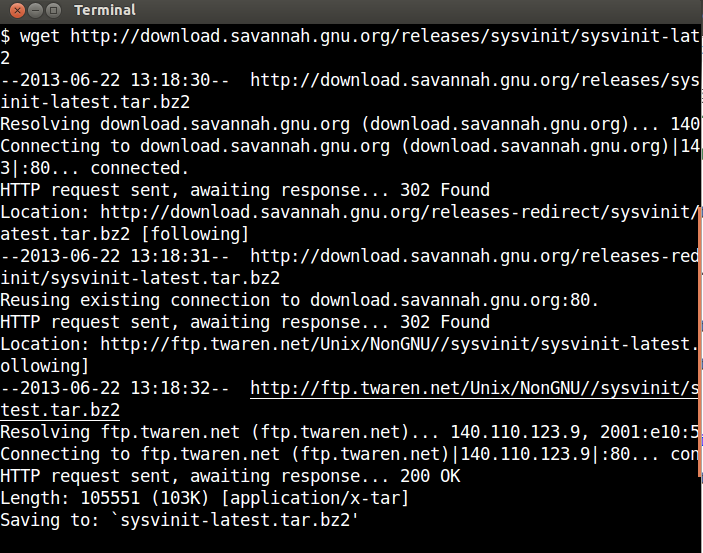
\includegraphics{./pictures/1-1-wget.png}
\caption{wget下载源码包}
\end{figure}

{\begin{shaded}\begin{verbatim}
$ wget http://download.savannah.gnu.org/releases/sysvinit/sysvinit-latest.tar.bz2
--2013-06-22 13:18:30--  http://download.savannah.gnu.org/releases/sysvinit/sysvinit-latest.tar.bz2
Resolving download.savannah.gnu.org (download.savannah.gnu.org)... 140.186.70.73
Connecting to download.savannah.gnu.org (download.savannah.gnu.org)|140.186.70.73|:80... connected.
HTTP request sent, awaiting response... 302 Found
Location: http://download.savannah.gnu.org/releases-redirect/sysvinit/sysvinit-latest.tar.bz2 [following]
--2013-06-22 13:18:31--  http://download.savannah.gnu.org/releases-redirect/sysvinit/sysvinit-latest.tar.bz2
Reusing existing connection to download.savannah.gnu.org:80.
HTTP request sent, awaiting response... 302 Found
Location: http://ftp.twaren.net/Unix/NonGNU//sysvinit/sysvinit-latest.tar.bz2 [following]
--2013-06-22 13:18:32--  http://ftp.twaren.net/Unix/NonGNU//sysvinit/sysvinit-latest.tar.bz2
Resolving ftp.twaren.net (ftp.twaren.net)... 140.110.123.9, 2001:e10:5c00:5::9
Connecting to ftp.twaren.net (ftp.twaren.net)|140.110.123.9|:80... connected.
HTTP request sent, awaiting response... 200 OK
Length: 105551 (103K) [application/x-tar]
Saving to: `sysvinit-latest.tar.bz2'

100%[======================================>] 105,551     45.1K/s   in 2.3s    

2013-06-22 13:18:35 (45.1 KB/s) - `sysvinit-latest.tar.bz2' saved [105551/105551]
\end{verbatim}\end{shaded}}
\subsection{tar解压源码包}

\begin{figure}[htbp]
\centering
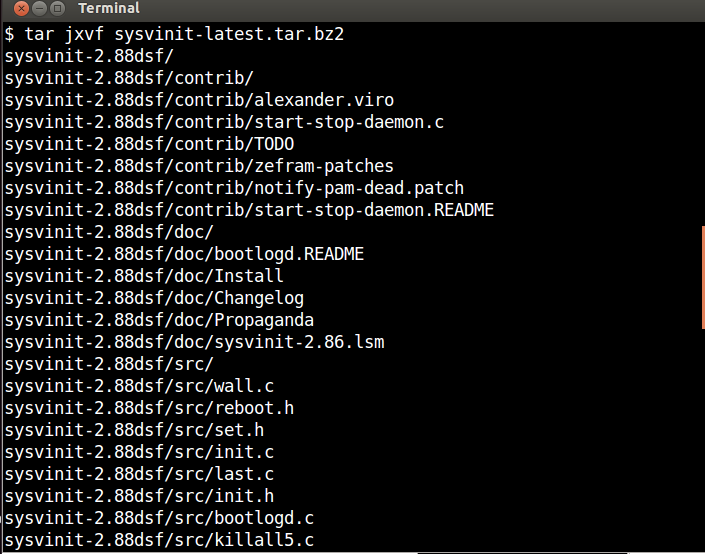
\includegraphics{./pictures/1-2-tar.png}
\caption{tar解压源码包}
\end{figure}

{\begin{shaded}\begin{verbatim}
$ tar jxvf sysvinit-latest.tar.bz2 
sysvinit-2.88dsf/
sysvinit-2.88dsf/contrib/
sysvinit-2.88dsf/contrib/alexander.viro
sysvinit-2.88dsf/contrib/start-stop-daemon.c
sysvinit-2.88dsf/contrib/TODO
sysvinit-2.88dsf/contrib/zefram-patches
sysvinit-2.88dsf/contrib/notify-pam-dead.patch
sysvinit-2.88dsf/contrib/start-stop-daemon.README
sysvinit-2.88dsf/doc/
sysvinit-2.88dsf/doc/bootlogd.README
sysvinit-2.88dsf/doc/Install
sysvinit-2.88dsf/doc/Changelog
sysvinit-2.88dsf/doc/Propaganda
sysvinit-2.88dsf/doc/sysvinit-2.86.lsm
sysvinit-2.88dsf/src/
sysvinit-2.88dsf/src/wall.c
sysvinit-2.88dsf/src/reboot.h
sysvinit-2.88dsf/src/set.h
sysvinit-2.88dsf/src/init.c
sysvinit-2.88dsf/src/last.c
sysvinit-2.88dsf/src/init.h
sysvinit-2.88dsf/src/bootlogd.c
sysvinit-2.88dsf/src/killall5.c
sysvinit-2.88dsf/src/utmpdump.c
sysvinit-2.88dsf/src/shutdown.c
sysvinit-2.88dsf/src/mountpoint.c
sysvinit-2.88dsf/src/sulogin.c
sysvinit-2.88dsf/src/fstab-decode.c
sysvinit-2.88dsf/src/initreq.h
sysvinit-2.88dsf/src/dowall.c
sysvinit-2.88dsf/src/hddown.c
sysvinit-2.88dsf/src/paths.h
sysvinit-2.88dsf/src/utmp.c
sysvinit-2.88dsf/src/ifdown.c
sysvinit-2.88dsf/src/initscript.sample
sysvinit-2.88dsf/src/halt.c
sysvinit-2.88dsf/src/oldutmp.h
sysvinit-2.88dsf/src/mesg.c
sysvinit-2.88dsf/src/Makefile
sysvinit-2.88dsf/src/runlevel.c
sysvinit-2.88dsf/COPYING
sysvinit-2.88dsf/COPYRIGHT
sysvinit-2.88dsf/man/
sysvinit-2.88dsf/man/bootlogd.8
sysvinit-2.88dsf/man/killall5.8
sysvinit-2.88dsf/man/shutdown.8
sysvinit-2.88dsf/man/bootlogd.8.todo
sysvinit-2.88dsf/man/sulogin.8
sysvinit-2.88dsf/man/fstab-decode.8
sysvinit-2.88dsf/man/mesg.1
sysvinit-2.88dsf/man/initscript.5
sysvinit-2.88dsf/man/inittab.5
sysvinit-2.88dsf/man/poweroff.8
sysvinit-2.88dsf/man/wall.1
sysvinit-2.88dsf/man/halt.8
sysvinit-2.88dsf/man/reboot.8
sysvinit-2.88dsf/man/last.1
sysvinit-2.88dsf/man/runlevel.8
sysvinit-2.88dsf/man/lastb.1
sysvinit-2.88dsf/man/pidof.8
sysvinit-2.88dsf/man/init.8
sysvinit-2.88dsf/man/utmpdump.1
sysvinit-2.88dsf/man/mountpoint.1
sysvinit-2.88dsf/man/telinit.8
sysvinit-2.88dsf/obsolete/
sysvinit-2.88dsf/obsolete/powerd.c
sysvinit-2.88dsf/obsolete/powerd.8
sysvinit-2.88dsf/obsolete/utmpdump.c.OLD
sysvinit-2.88dsf/obsolete/README.RIGHT.NOW
sysvinit-2.88dsf/obsolete/bootlogd.init
sysvinit-2.88dsf/obsolete/powerd.README
sysvinit-2.88dsf/obsolete/powerd.cfg
sysvinit-2.88dsf/Makefile
sysvinit-2.88dsf/README
$ 

$ ls
Makefile  pdf  sysvinit-2.88dsf  sysvinit-latest.tar.bz2

$ ls sysvinit-2.88dsf/
contrib  COPYRIGHT  Makefile  obsolete  src
COPYING  doc        man       README
$ 
\end{verbatim}\end{shaded}}
\subsection{编译项目源码}

{\begin{shaded}\begin{verbatim}
$ cd sysvinit-2.88dsf/
$ make
cc -ansi -O2 -fomit-frame-pointer -W -Wall -D_GNU_SOURCE   -c -o mountpoint.o mountpoint.c
cc   mountpoint.o   -o mountpoint
cc -ansi -O2 -fomit-frame-pointer -W -Wall -D_GNU_SOURCE   -c -o init.o init.c
init.c: In function ‘telinit’:
init.c:2737:7: warning: ignoring return value of ‘chdir’, declared with attribute warn_unused_result [-Wunused-result]
init.c: In function ‘get_record’:
init.c:377:11: warning: ignoring return value of ‘fscanf’, declared with attribute warn_unused_result [-Wunused-result]
init.c:380:11: warning: ignoring return value of ‘fscanf’, declared with attribute warn_unused_result [-Wunused-result]
init.c:383:11: warning: ignoring return value of ‘fscanf’, declared with attribute warn_unused_result [-Wunused-result]
init.c:386:11: warning: ignoring return value of ‘fscanf’, declared with attribute warn_unused_result [-Wunused-result]
init.c:389:11: warning: ignoring return value of ‘fscanf’, declared with attribute warn_unused_result [-Wunused-result]
init.c:392:11: warning: ignoring return value of ‘fscanf’, declared with attribute warn_unused_result [-Wunused-result]
init.c:395:11: warning: ignoring return value of ‘fscanf’, declared with attribute warn_unused_result [-Wunused-result]
init.c:398:11: warning: ignoring return value of ‘fscanf’, declared with attribute warn_unused_result [-Wunused-result]
init.c:401:11: warning: ignoring return value of ‘fscanf’, declared with attribute warn_unused_result [-Wunused-result]
init.c:404:11: warning: ignoring return value of ‘fscanf’, declared with attribute warn_unused_result [-Wunused-result]
init.c:423:10: warning: ignoring return value of ‘fscanf’, declared with attribute warn_unused_result [-Wunused-result]
init.c:426:10: warning: ignoring return value of ‘fscanf’, declared with attribute warn_unused_result [-Wunused-result]
init.c: In function ‘spawn’:
init.c:1064:10: warning: ignoring return value of ‘dup’, declared with attribute warn_unused_result [-Wunused-result]
init.c:1065:10: warning: ignoring return value of ‘dup’, declared with attribute warn_unused_result [-Wunused-result]
init.c:1133:7: warning: ignoring return value of ‘dup’, declared with attribute warn_unused_result [-Wunused-result]
init.c:1134:7: warning: ignoring return value of ‘dup’, declared with attribute warn_unused_result [-Wunused-result]
init.c: In function ‘ask_runlevel’:
init.c:1673:10: warning: ignoring return value of ‘write’, declared with attribute warn_unused_result [-Wunused-result]
init.c:1675:9: warning: ignoring return value of ‘read’, declared with attribute warn_unused_result [-Wunused-result]
init.c: In function ‘make_pipe’:
init.c:1960:6: warning: ignoring return value of ‘pipe’, declared with attribute warn_unused_result [-Wunused-result]
init.c:1965:7: warning: ignoring return value of ‘write’, declared with attribute warn_unused_result [-Wunused-result]
init.c: In function ‘process_signals’:
init.c:2411:7: warning: ignoring return value of ‘read’, declared with attribute warn_unused_result [-Wunused-result]
init.c:2420:7: warning: ignoring return value of ‘read’, declared with attribute warn_unused_result [-Wunused-result]
init.c: In function ‘coredump’:
init.c:666:7: warning: ignoring return value of ‘chdir’, declared with attribute warn_unused_result [-Wunused-result]
init.c: In function ‘print’:
init.c:821:8: warning: ignoring return value of ‘write’, declared with attribute warn_unused_result [-Wunused-result]
cc -ansi -O2 -fomit-frame-pointer -W -Wall -D_GNU_SOURCE -DINIT_MAIN -c -o init_utmp.o utmp.c
cc   init.o init_utmp.o    -o init
cc -ansi -O2 -fomit-frame-pointer -W -Wall -D_GNU_SOURCE   -c -o halt.o halt.c
halt.c: In function ‘main’:
halt.c:242:2: warning: ignoring return value of ‘chdir’, declared with attribute warn_unused_result [-Wunused-result]
cc -ansi -O2 -fomit-frame-pointer -W -Wall -D_GNU_SOURCE   -c -o ifdown.o ifdown.c
cc -ansi -O2 -fomit-frame-pointer -W -Wall -D_GNU_SOURCE   -c -o hddown.o hddown.c
cc -ansi -O2 -fomit-frame-pointer -W -Wall -D_GNU_SOURCE   -c -o utmp.o utmp.c
cc   halt.o ifdown.o hddown.o utmp.o reboot.h   -o halt
cc -ansi -O2 -fomit-frame-pointer -W -Wall -D_GNU_SOURCE   -c -o shutdown.o shutdown.c
shutdown.c: In function ‘main’:
shutdown.c:485:10: warning: variable ‘realuid’ set but not used [-Wunused-but-set-variable]
shutdown.c:630:9: warning: ignoring return value of ‘fscanf’, declared with attribute warn_unused_result [-Wunused-result]
shutdown.c:719:7: warning: ignoring return value of ‘chdir’, declared with attribute warn_unused_result [-Wunused-result]
shutdown.c: In function ‘spawn’:
shutdown.c:289:7: warning: ignoring return value of ‘chdir’, declared with attribute warn_unused_result [-Wunused-result]
cc -ansi -O2 -fomit-frame-pointer -W -Wall -D_GNU_SOURCE   -c -o dowall.o dowall.c
cc   shutdown.o dowall.o utmp.o reboot.h   -o shutdown
cc -ansi -O2 -fomit-frame-pointer -W -Wall -D_GNU_SOURCE   -c -o runlevel.o runlevel.c
cc   runlevel.o   -o runlevel
cc -ansi -O2 -fomit-frame-pointer -W -Wall -D_GNU_SOURCE   -c -o sulogin.o sulogin.c
sulogin.c: In function ‘sushell’:
sulogin.c:407:2: warning: ignoring return value of ‘chdir’, declared with attribute warn_unused_result [-Wunused-result]
sulogin.c:427:8: warning: ignoring return value of ‘getcwd’, declared with attribute warn_unused_result [-Wunused-result]
cc   sulogin.o    -o sulogin
sulogin.o: In function `main':
sulogin.c:(.text.startup+0x1e2): undefined reference to `crypt'
collect2: ld returned 1 exit status
make: *** [sulogin] Error 1
$ 
\end{verbatim}\end{shaded}}
\subsection{修改 Makefile 使之能够编译通过}

\begin{figure}[htbp]
\centering
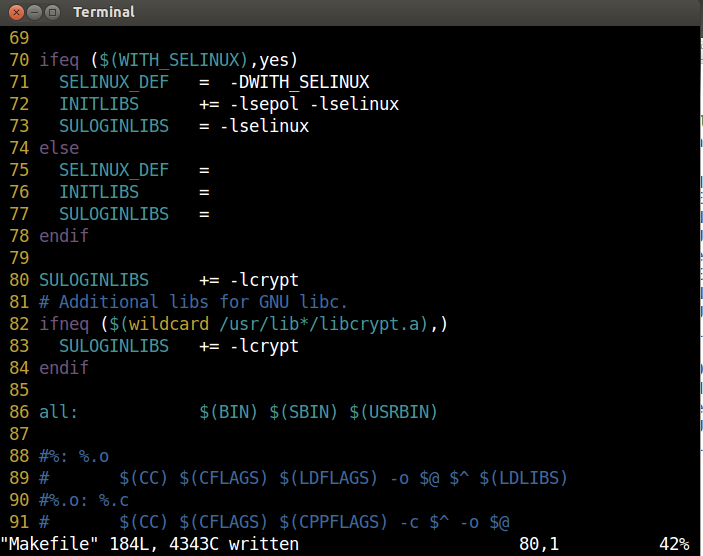
\includegraphics{./pictures/1-3-makefile.png}
\caption{修改 Makefile}
\end{figure}

{\begin{shaded}\begin{verbatim}
$ vi Makefile 
69 
70 ifeq ($(WITH_SELINUX),yes)
71   SELINUX_DEF   =  -DWITH_SELINUX
72   INITLIBS      += -lsepol -lselinux
73   SULOGINLIBS   = -lselinux
74 else
75   SELINUX_DEF   =
76   INITLIBS      =
77   SULOGINLIBS   =
78 endif
79 
80 SULOGINLIBS     += -lcrypt
81 # Additional libs for GNU libc.
82 ifneq ($(wildcard /usr/lib*/libcrypt.a),)
83   SULOGINLIBS   += -lcrypt
84 endif
85 
86 all:            $(BIN) $(SBIN) $(USRBIN)
87 
88 #%: %.o
89 #       $(CC) $(CFLAGS) $(LDFLAGS) -o $@ $^ $(LDLIBS)
90 #%.o: %.c
91 #       $(CC) $(CFLAGS) $(CPPFLAGS) -c $^ -o $@
\end{verbatim}\end{shaded}}
在80行处添加83行处的赋值,增加链接时 -lcrypt 选项

\subsection{继续编译项目源码,成功}

\begin{figure}[htbp]
\centering
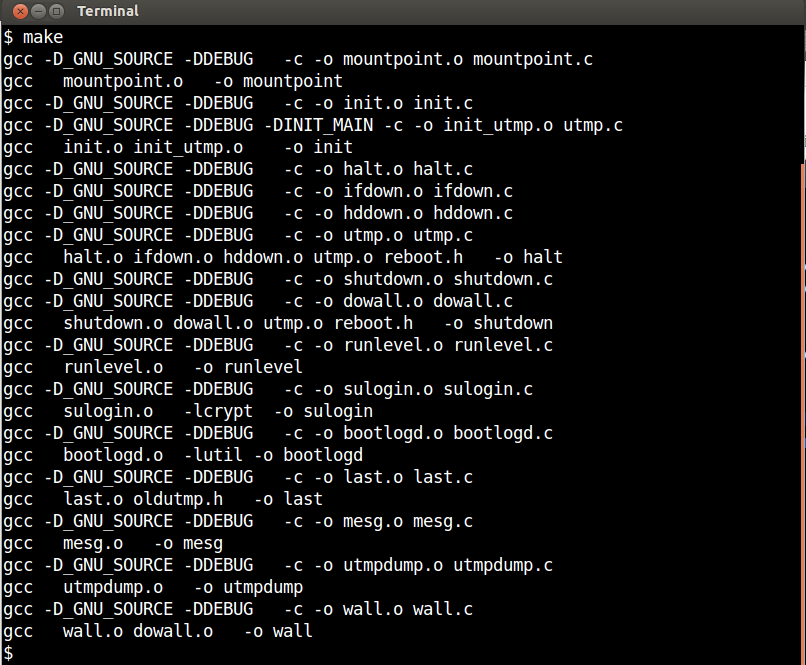
\includegraphics{./pictures/1-4-make.png}
\caption{make编译源码包}
\end{figure}

{\begin{shaded}\begin{verbatim}
$ make
cc   sulogin.o   -lcrypt  -o sulogin
cc -ansi -O2 -fomit-frame-pointer -W -Wall -D_GNU_SOURCE   -c -o bootlogd.o bootlogd.c
bootlogd.c: In function ‘findtty’:
bootlogd.c:125:8: warning: ignoring return value of ‘chdir’, declared with attribute warn_unused_result [-Wunused-result]
bootlogd.c:140:10: warning: ignoring return value of ‘chdir’, declared with attribute warn_unused_result [-Wunused-result]
bootlogd.c:151:10: warning: ignoring return value of ‘chdir’, declared with attribute warn_unused_result [-Wunused-result]
bootlogd.c:156:10: warning: ignoring return value of ‘chdir’, declared with attribute warn_unused_result [-Wunused-result]
bootlogd.c:163:7: warning: ignoring return value of ‘chdir’, declared with attribute warn_unused_result [-Wunused-result]
cc   bootlogd.o  -lutil -o bootlogd
cc -ansi -O2 -fomit-frame-pointer -W -Wall -D_GNU_SOURCE   -c -o last.o last.c
cc   last.o oldutmp.h   -o last
cc -ansi -O2 -fomit-frame-pointer -W -Wall -D_GNU_SOURCE   -c -o mesg.o mesg.c
cc   mesg.o   -o mesg
cc -ansi -O2 -fomit-frame-pointer -W -Wall -D_GNU_SOURCE   -c -o utmpdump.o utmpdump.c
cc   utmpdump.o   -o utmpdump
cc -ansi -O2 -fomit-frame-pointer -W -Wall -D_GNU_SOURCE   -c -o wall.o wall.c
cc   wall.o dowall.o   -o wall
$ 
\end{verbatim}\end{shaded}}
\subsection{查看生成的可执行文件}

\begin{figure}[htbp]
\centering
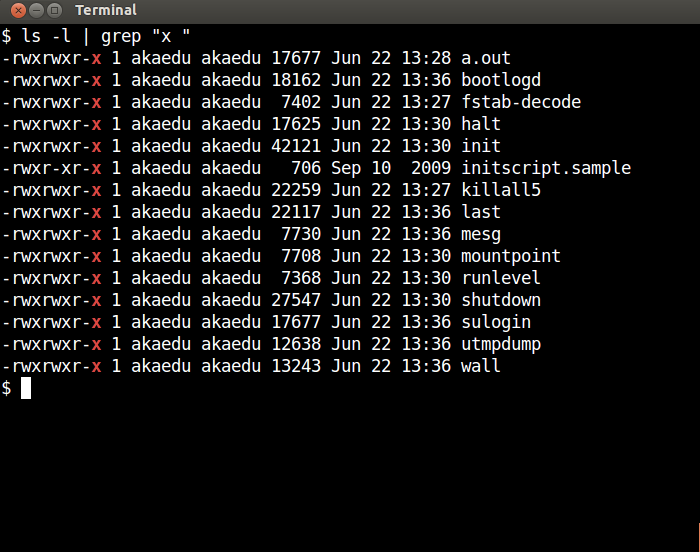
\includegraphics{./pictures/1-5-executables.png}
\caption{查看可执行文件}
\end{figure}

{\begin{shaded}\begin{verbatim}
$ ls -l | grep "x "
-rwxrwxr-x 1 akaedu akaedu 17677 Jun 22 13:28 a.out
-rwxrwxr-x 1 akaedu akaedu 18162 Jun 22 13:36 bootlogd
-rwxrwxr-x 1 akaedu akaedu  7402 Jun 22 13:27 fstab-decode
-rwxrwxr-x 1 akaedu akaedu 17625 Jun 22 13:30 halt
-rwxrwxr-x 1 akaedu akaedu 42121 Jun 22 13:30 init
-rwxr-xr-x 1 akaedu akaedu   706 Sep 10  2009 initscript.sample
-rwxrwxr-x 1 akaedu akaedu 22259 Jun 22 13:27 killall5
-rwxrwxr-x 1 akaedu akaedu 22117 Jun 22 13:36 last
-rwxrwxr-x 1 akaedu akaedu  7730 Jun 22 13:36 mesg
-rwxrwxr-x 1 akaedu akaedu  7708 Jun 22 13:30 mountpoint
-rwxrwxr-x 1 akaedu akaedu  7368 Jun 22 13:30 runlevel
-rwxrwxr-x 1 akaedu akaedu 27547 Jun 22 13:30 shutdown
-rwxrwxr-x 1 akaedu akaedu 17677 Jun 22 13:36 sulogin
-rwxrwxr-x 1 akaedu akaedu 12638 Jun 22 13:36 utmpdump
-rwxrwxr-x 1 akaedu akaedu 13243 Jun 22 13:36 wall
$ 
\end{verbatim}\end{shaded}}
\section{Linux 内核启动 init 进程}

\subsection{start\_kernel}

{\begin{shaded}\begin{verbatim}
545 asmlinkage void __init start_kernel(void)
546 {
547         char * command_line;
548         unsigned long mempages;
549         extern char saved_command_line[];
550 /*
551  * Interrupts are still disabled. Do necessary setups, then
552  * enable them
553  */
554         lock_kernel();
555         printk(linux_banner);
556         setup_arch(&command_line);
557         printk("Kernel command line: %s\n", saved_command_line);
558         parse_options(command_line);
559         trap_init();
560         init_IRQ();
561         sched_init();
562         softirq_init();
563         time_init();
564 
.....
622         /* 
623          *      We count on the initial thread going ok 
624          *      Like idlers init is an unlocked kernel thread, which will
625          *      make syscalls (and thus be locked).
626          */
627         smp_init();
628         rest_init();
629 }
630 
\end{verbatim}\end{shaded}}
\begin{figure}[htbp]
\centering
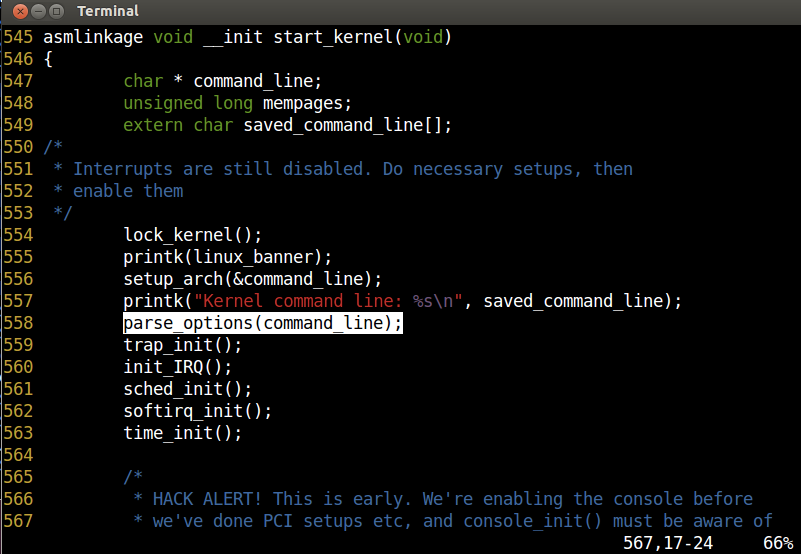
\includegraphics{./pictures/start_kernel.png}
\caption{内核start\_kernel函数}
\end{figure}

\subsection{parse\_options}

{\begin{shaded}\begin{verbatim}
426 static void __init parse_options(char *line)
427 {
428         char *next,*quote;
429         int args, envs;
430 
431         if (!*line)
432                 return;
433         args = 0;
434         envs = 1;       /* TERM is set to 'linux' by default */
435         next = line;
436         while ((line = next) != NULL) {
437                 quote = strchr(line,'"');
438                 next = strchr(line, ' ');
439                 while (next != NULL && quote != NULL && quote < next) {
440                         /* we found a left quote before the next blank
441                          * now we have to find the matching right quote
442                          */
443                         next = strchr(quote+1, '"');
444                         if (next != NULL) {
445                                 quote = strchr(next+1, '"');
446                                 next = strchr(next+1, ' ');
447                         }
448                 }
449                 if (next != NULL)
450                         *next++ = 0;
451                 if (!strncmp(line,"init=",5)) {
452                         line += 5;
453                         execute_command = line;
454                         /* In case LILO is going to boot us with default com      
\end{verbatim}\end{shaded}}
\begin{figure}[htbp]
\centering
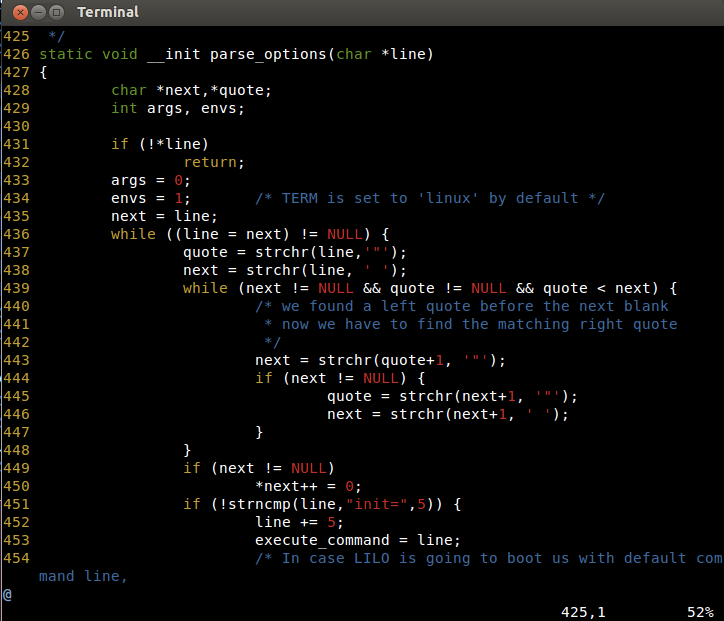
\includegraphics{./pictures/parse_options.png}
\caption{内核parse\_options函数}
\end{figure}

\subsection{rest\_init}

{\begin{shaded}\begin{verbatim}
532 
533 static void rest_init(void)
534 {
535         kernel_thread(init, NULL, CLONE_FS | CLONE_FILES | CLONE_SIGNAL);
536         unlock_kernel();
537         current->need_resched = 1;
538         cpu_idle();
539 }
540 
\end{verbatim}\end{shaded}}
\subsection{init 函数}

{\begin{shaded}\begin{verbatim}
805 static int init(void * unused)
806 {
807         lock_kernel();
808         do_basic_setup();
809 
810         prepare_namespace();
811 
812         /*
813          * Ok, we have completed the initial bootup, and
814          * we're essentially up and running. Get rid of the
815          * initmem segments and start the user-mode stuff..
816          */
817         free_initmem();
818         unlock_kernel();
819 
820         if (open("/dev/console", O_RDWR, 0) < 0)
821                 printk("Warning: unable to open an initial console.\n");
822 
823         (void) dup(0);
824         (void) dup(0);
825 
826         /*
827          * We try each of these until one succeeds.
828          *
829          * The Bourne shell can be used instead of init if we are 
830          * trying to recover a really broken machine.
831          */
832 
833         if (execute_command)
834                 execve(execute_command,argv_init,envp_init);
835         execve("/sbin/init",argv_init,envp_init);
836         execve("/etc/init",argv_init,envp_init);
837         execve("/bin/init",argv_init,envp_init);
838         execve("/bin/sh",argv_init,envp_init);
839         panic("No init found.  Try passing init= option to kernel.");
840 }
\end{verbatim}\end{shaded}}
\begin{figure}[htbp]
\centering
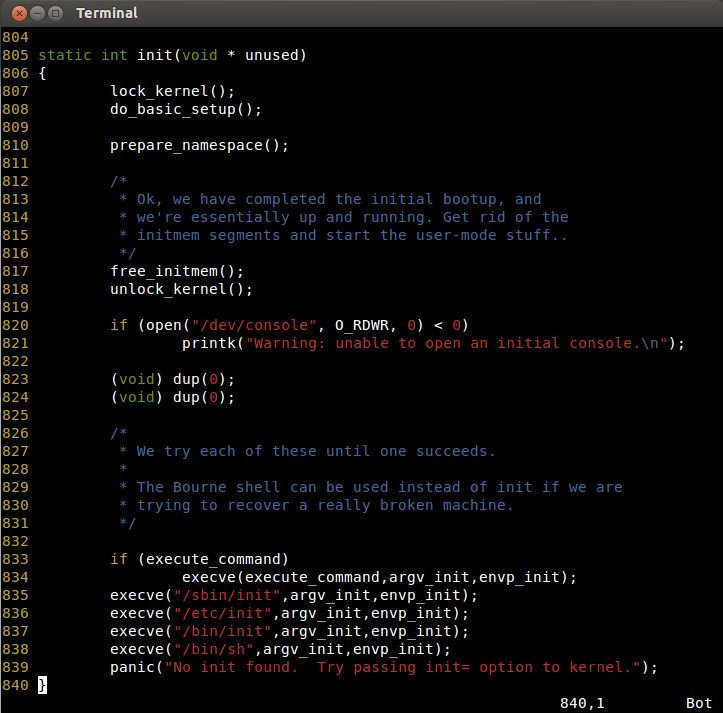
\includegraphics{./pictures/init.png}
\caption{内核init函数}
\end{figure}

至此我们找到了一条路径,使得内核从 start\_kernel 的主函数,进入到 init
进程。这里涉及到了4个重要的函数和1个重要的变量,这些都是和 init
进程如何启动直接相关的,对于我们了解在 init
进程启动之前的逻辑流程有重要作用。

\begin{itemize}
\item
  start\_kernel()
\item
  parse\_options()
\item
  rest\_init()
\item
  init()
\item
  execute\_command
\end{itemize}
我们用下面这张图来表示这些函数和变量之间的关系,可以更直观的看到内核启动init进程的流程。

\begin{figure}[htbp]
\centering
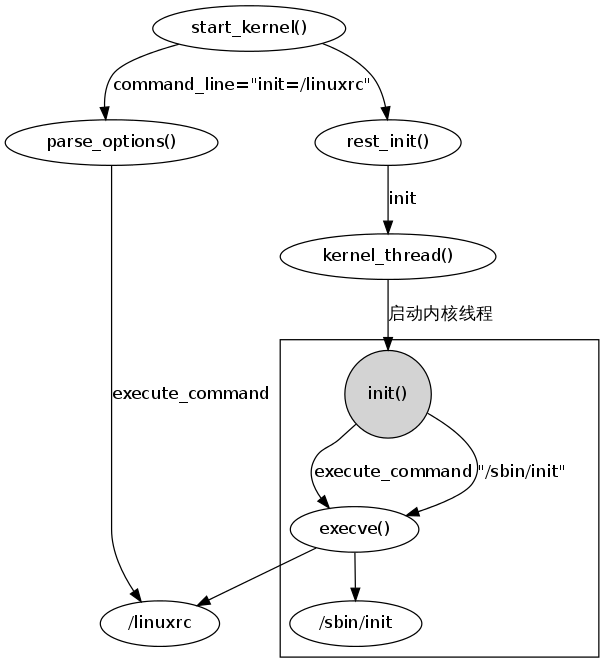
\includegraphics{./figures/kernel2init.png}
\caption{Linux 内核启动 init 进程}
\end{figure}

\subsubsection{/sbin/init}

